%%%%%%%%%%%%%%%%%%%%%%%%%%%%%%%%%%%%%%%%%%%%%%%%%%%%%%%%%%%%%%%%%%%%%%%%%%%%%%%%%%%%%%%%%%%%%%%%
%
% CSCI 1430 Written Question Template
%
% This is a LaTeX document. LaTeX is a markup language for producing documents.
% Your task is to answer the questions by filling out this document, then to
% compile this into a PDF document.

%
%
% TO COMPILE:
% > pdflatex thisfile.tex
%
% If you do not have LaTeX and need a LaTeX distribution:
% - Departmental machines have one installed.
% - Personal laptops (all common OS): http://www.latex-project.org/get/
%
% If you need help with LaTeX, come to office hours. Or, there is plenty of help online:
% https://en.wikibooks.org/wiki/LaTeX
%
% Good luck!
% James and the 1430 staff
%
%%%%%%%%%%%%%%%%%%%%%%%%%%%%%%%%%%%%%%%%%%%%%%%%%%%%%%%%%%%%%%%%%%%%%%%%%%%%%%%%%%%%%%%%%%%%%%%%
%
% How to include two graphics on the same line:
%
% \includegraphics[width=0.49\linewidth]{yourgraphic1.png}
% \includegraphics[width=0.49\linewidth]{yourgraphic2.png}
%
% How to include equations:
%
% \begin{equation}
% y = mx+c
% \end{equation}
%
%%%%%%%%%%%%%%%%%%%%%%%%%%%%%%%%%%%%%%%%%%%%%%%%%%%%%%%%%%%%%%%%%%%%%%%%%%%%%%%%%%%%%%%%%%%%%%%%

\documentclass[11pt]{article}

\usepackage[english]{babel}
\usepackage[utf8]{inputenc}
\usepackage[colorlinks = true,
            linkcolor = blue,
            urlcolor  = blue]{hyperref}
\usepackage[a4paper,margin=1.5in]{geometry}
\usepackage{stackengine,graphicx}
\usepackage{fancyhdr}
\setlength{\headheight}{15pt}
\usepackage{microtype}
\usepackage{times}
\usepackage{listings}

\frenchspacing
\setlength{\parindent}{0cm} % Default is 15pt.
\setlength{\parskip}{0.3cm plus1mm minus1mm}

\pagestyle{fancy}
\fancyhf{}
\lhead{Project 1 Questions}
\rhead{CIE552}
\rfoot{\thepage}

\date{}

\title{\vspace{-1cm}Project 1 Questions}


\begin{document}
\maketitle
\vspace{-3cm}
\thispagestyle{fancy}

\section*{Instructions}
\begin{itemize}
  \item 4 questions.
  \item Write code where appropriate.
  \item Feel free to include images or equations.
\end{itemize}

\section*{Questions}

\paragraph{Q1:} Explicitly describe image convolution: the input, the transformation, and the output. Why is it useful for computer vision?

%%%%%%%%%%%%%%%%%%%%%%%%%%%%%%%%%%%
\paragraph{A1:} Image convolution is a mathematical operation that includes multiplication and addition. Two matrices, one of which has to have odd dimensions( The kernel ), are used as input in the operations most basic form. For each pixel i, convolution adds the pixel value with its neighbouring pixels, all of which are weighted by the kernel. The process is iteratively repeated for every pixel. As for the output, given two matrices of dimensions $M\times N$ and $K\times L$, the output is a matrix of the size $(M+K-1)\times (N+L-1)$.Convolution is an essential tool in Computer vision since it can be used to transform the matrix in a way that allows objects edges only to be seen and therefore help in the detection and identification of said objects( edge detection, sobel and emboss filters ). Convolution can also be used to enhance images in several ways such as sharpening, noise removal, and blurring, which can be useful in specific applications such as computational photography and aiding with scene and color detection in mobile phones.



%%%%%%%%%%%%%%%%%%%%%%%%%%%%%%%%%%%

% Please leave the pagebreak
\pagebreak
\paragraph{Q2:} What is the difference between convolution and correlation? Construct a scenario which produces a different output between both operations.

\emph{Please use \href{https://docs.scipy.org/doc/scipy/reference/generated/scipy.ndimage.convolve.html}{$scipy.ndimage.convolve$} and \href{https://docs.scipy.org/doc/scipy/reference/generated/scipy.ndimage.correlate.html}{$scipy.ndimage.correlate$} to experiment!}

%%%%%%%%%%%%%%%%%%%%%%%%%%%%%%%%%%%
\paragraph{A2:} Convolution and Correlation preform the same multiplication and addition operations on matrices, with the only difference being that the kernel is flipped in convolution before addition and multiplication. In correlation no flipping occurs. This means that convolving one image with another using \href{https://docs.scipy.org/doc/scipy/reference/generated/scipy.ndimage.convolve.html}{$scipy.ndimage.convolve$} and correlating the two images using \href{https://docs.scipy.org/doc/scipy/reference/generated/scipy.ndimage.correlate.html}{$scipy.ndimage.correlate$} with one being already flipped should result in the same output. Usually convolution and correlation also produce the same output when the kernel is symmetric, as flipping a symmetric kernel results in no change. A good scenario where convolution and correlation produce different results is when an image is correlated and convolved with a right sobel kernel. A typical right sobel matrix is as follows:
\begin{center}
  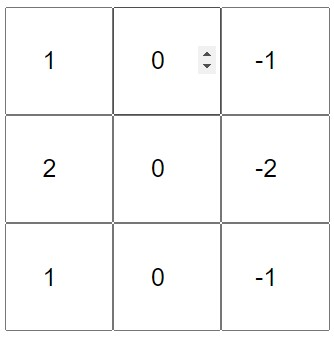
\includegraphics[scale=0.5]{matrix.jpg}  
\end{center}
\paragraph {}If the kernel above was used in both correlation and convolution the convolution result would be equivalent to a left sobel correlation.
\begin{table}[h!]
     \begin{center}
     \begin{tabular}{c c c c}
      Correlation & Convolution \\ 
     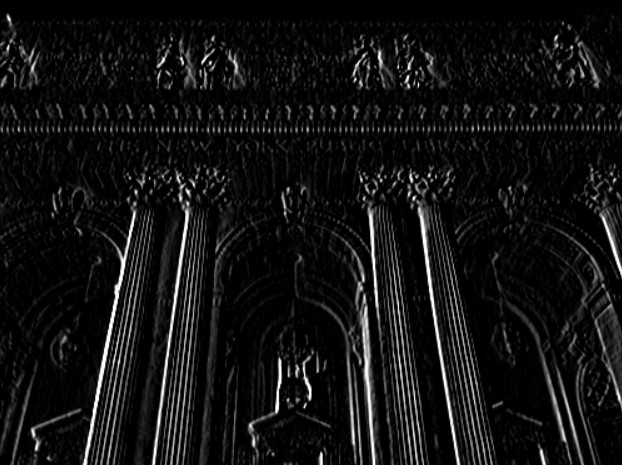
\includegraphics[scale=0.5]{right.jpg}
      & 
      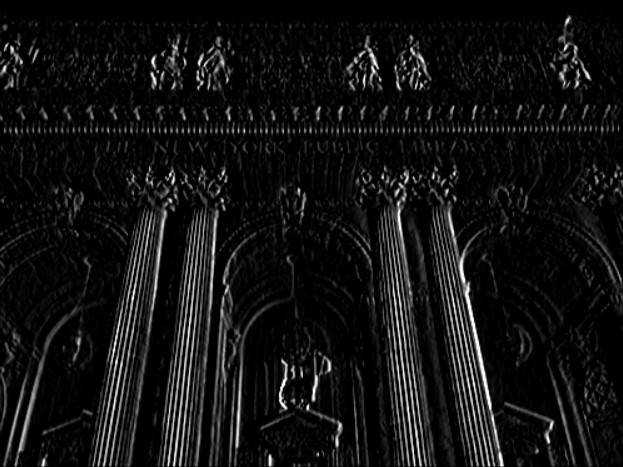
\includegraphics[scale=0.5]{leftsobel.jpg}
      \end{tabular}
      \end{center}
      \end{table}



%%%%%%%%%%%%%%%%%%%%%%%%%%%%%%%%%%%

% Please leave the pagebreak
\pagebreak
\paragraph{Q3:} What is the difference between a high pass filter and a low pass filter in how they are constructed, and what they do to the image? Please provide example kernels and output images.

%%%%%%%%%%%%%%%%%%%%%%%%%%%%%%%%%%%
\paragraph{A3:}
\paragraph{  }A low pass filter is constructed by creating a 2-dimensional Gaussian matrix or by creating a mean filter through dividing a matrix of ones by the number of elements inside said matrix. This causes the value for each pixel to be influenced by its neighbours in decreasing amount as the neighbour gets more distant, or equally by all neighbours respectively. The output of applying the mean or Gaussian filter to an image is a blurry copy of the original.

\paragraph{  }A high pass filter is constructed by creating a 2-dimensional Laplacian matrix or creating an edge detection matrix in which all elements but the core of the kernel are negatives, while the core is positive and scaled accordingly. This causes the value for each output pixel to only be bright enough when sudden changes in brightness occur between each pixel and its neighbours. The output of applying a high pass filter is usually an image where only the edges are visible and it is usually used in edge detection.

\paragraph{}
\begin{table}[h!]
     \begin{center}
     \begin{tabular}{c c c c}
      Low pass filter & High pass filter \\ 
     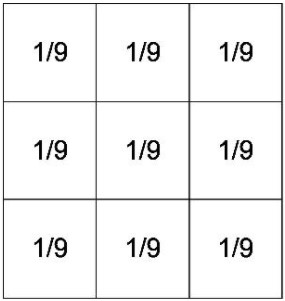
\includegraphics[scale=0.7]{lpf.jpg}
      & 
      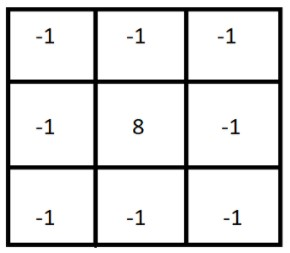
\includegraphics[scale=0.7]{hpf.jpg}\\
      Low pass image output & High pass image output \\ 
      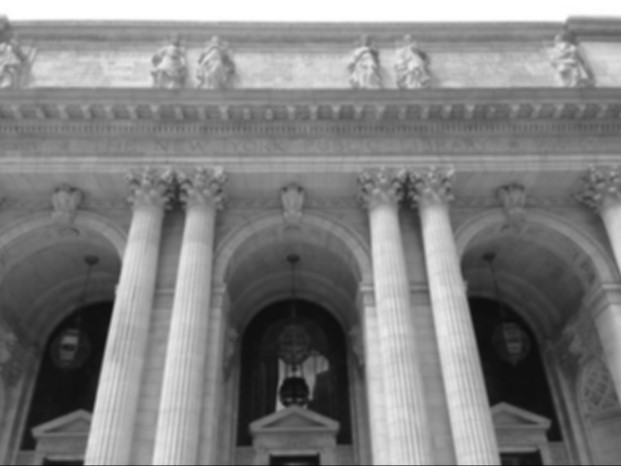
\includegraphics[scale=0.4]{lpres.jpg}
      & 
      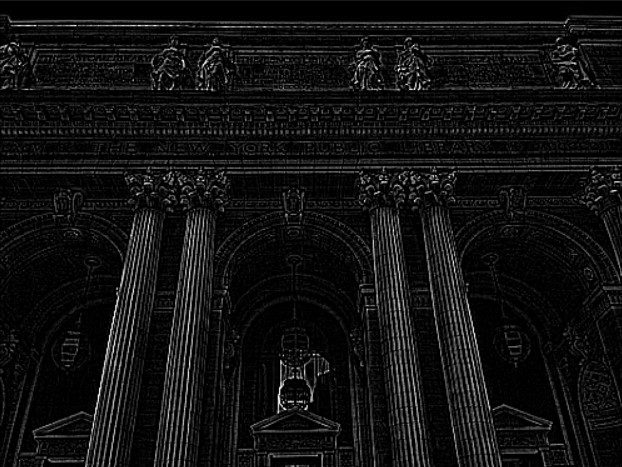
\includegraphics[scale=0.4]{hpres.jpg}
      \end{tabular}
      \end{center}
      \end{table}





%%%%%%%%%%%%%%%%%%%%%%%%%%%%%%%%%%%

% Please leave the pagebreak
\pagebreak
\paragraph{Q4:} How does computation time vary with filter sizes from $3\times3$ to $15\times15$ (for all odd and square sizes), and with image sizes from 0.25~MPix to 8~MPix (choose your own intervals)? Measure both using \href{https://docs.scipy.org/doc/scipy/reference/generated/scipy.ndimage.convolve.html}{$scipy.ndimage.convolve$} or \href{https://docs.scipy.org/doc/scipy/reference/generated/scipy.ndimage.correlate.html}{$scipy.ndimage.correlate$} to produce a matrix of values. Use the \href{http://scikit-image.org/docs/dev/auto_examples/transform/plot_rescale.html}{$skimage.transform$} module to vary the size of an image. Use an appropriate charting function to plot your matrix of results, such as \href{https://matplotlib.org/tutorials/toolkits/mplot3d.html#scatter-plots}{$Axes3D.scatter$} or \href{https://matplotlib.org/tutorials/toolkits/mplot3d.html#surface-plots}{$Axes3D.plot\textrm{\_}surface$}.

Do the results match your expectation given the number of multiply and add operations in convolution?

\emph{Image:} \href{RISDance.jpg}{RISDance.jpg} (in the project directory).

%%%%%%%%%%%%%%%%%%%%%%%%%%%%%%%%%%%
\paragraph{A4:} for each iteration in the convolution process, for a kernel with size $N\times N$, with $N$ being an odd value ranging from 3 to 15, $N\times N$ multiplications are made and  $(N\times N-1)$ additions follow. This repeats for each pixel in the other image, which means it repeats K times with K ranging from $0.25\times10^{6}$ to $8\times10^{6}$

\paragraph{Matrix of Results: }
\begin{center}
    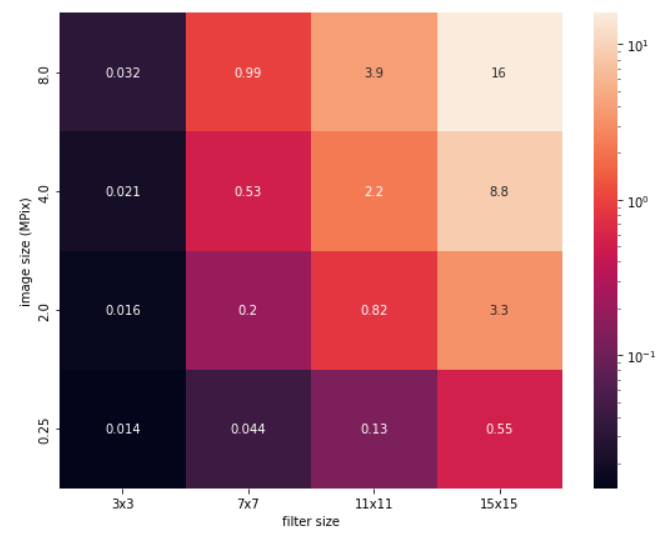
\includegraphics[scale=0.5]{image.png}
\end{center}
\pagebreak

\paragraph{Code }:

\begin{lstlisting}[language=Python]

from scipy.signal import convolve2d, correlate2d
import numpy as np
import cv2
from matplotlib import pyplot as plt
from scipy import ndimage
from skimage.transform import rescale
import time
import seaborn as sn
from matplotlib.colors import LogNorm, Normalize


img = cv2.imread('RISDance.jpg')
plt.imshow(cv2.cvtColor(img, cv2.COLOR_BGR2RGB)) ;

imgsize = (img.shape[0]*img.shape[1])/(10**6)
sizes=np.array([0.25 ,2, 4, 8])
ratio=sizes/imgsize

img0= rescale(img, ratio[0], mode='reflect', multichannel=True)
img1= rescale(img, ratio[1], mode='reflect', multichannel=True)
img2= rescale(img, ratio[2], mode='reflect', multichannel=True)
img3= rescale(img, ratio[3], mode='reflect', multichannel=True)

def create_mean_filter(ksize):
    assert ksize % 2 != 0
    mean_filter = np.ones((ksize, ksize, 3), dtype=np.uint8) * (1/(ksize**2))
    return mean_filter
    
kernel0 = create_mean_filter(3)
kernel1 = create_mean_filter(7)
kernel2 = create_mean_filter(11)
kernel3 = create_mean_filter(15)

imglist= [img0, img1, img2, img3]
kernellist=[kernel0, kernel1, kernel2, kernel3 ]

exec_time = np.ndarray((4,4))
for i in range(4):
    for j in range (4):
        imgtmp,kerneltmp=imglist[j],kernellist[i]
        start_time = time.time()
        output = ndimage.convolve(imgtmp,kerneltmp, mode ='constant')
        endtime = time.time() - start_time
        exec_time[i,j]=endtime

plt.figure(figsize=(9,7));
hm = sn.heatmap(data=exec_time, annot=True,norm=LogNorm())
hm.invert_yaxis()
hm.set_xticklabels(['3x3','7x7','11x11','15x15'])
hm.set_xlabel('filter size')
hm.set_yticklabels(sizes)
hm.set_ylabel('image size (MPix)')
plt.show();
\end{lstlisting}


%%%%%%%%%%%%%%%%%%%%%%%%%%%%%%%%%%%


% If you really need extra space, uncomment here and use extra pages after the last question.
% Please refer here in your original answer. Thanks!
%\pagebreak
%\paragraph{AX.X Continued:} Your answer continued here.



\end{document}
